% Options for packages loaded elsewhere
\PassOptionsToPackage{unicode}{hyperref}
\PassOptionsToPackage{hyphens}{url}
%
\documentclass[
  12pt,
]{article}
\usepackage{amsmath,amssymb}
\usepackage{iftex}
\ifPDFTeX
  \usepackage[T1]{fontenc}
  \usepackage[utf8]{inputenc}
  \usepackage{textcomp} % provide euro and other symbols
\else % if luatex or xetex
  \usepackage{unicode-math} % this also loads fontspec
  \defaultfontfeatures{Scale=MatchLowercase}
  \defaultfontfeatures[\rmfamily]{Ligatures=TeX,Scale=1}
\fi
\usepackage{lmodern}
\ifPDFTeX\else
  % xetex/luatex font selection
\fi
% Use upquote if available, for straight quotes in verbatim environments
\IfFileExists{upquote.sty}{\usepackage{upquote}}{}
\IfFileExists{microtype.sty}{% use microtype if available
  \usepackage[]{microtype}
  \UseMicrotypeSet[protrusion]{basicmath} % disable protrusion for tt fonts
}{}
\makeatletter
\@ifundefined{KOMAClassName}{% if non-KOMA class
  \IfFileExists{parskip.sty}{%
    \usepackage{parskip}
  }{% else
    \setlength{\parindent}{0pt}
    \setlength{\parskip}{6pt plus 2pt minus 1pt}}
}{% if KOMA class
  \KOMAoptions{parskip=half}}
\makeatother
\usepackage{xcolor}
\usepackage[a4paper]{geometry}
\usepackage{color}
\usepackage{fancyvrb}
\newcommand{\VerbBar}{|}
\newcommand{\VERB}{\Verb[commandchars=\\\{\}]}
\DefineVerbatimEnvironment{Highlighting}{Verbatim}{commandchars=\\\{\}}
% Add ',fontsize=\small' for more characters per line
\usepackage{framed}
\definecolor{shadecolor}{RGB}{248,248,248}
\newenvironment{Shaded}{\begin{snugshade}}{\end{snugshade}}
\newcommand{\AlertTok}[1]{\textcolor[rgb]{0.94,0.16,0.16}{#1}}
\newcommand{\AnnotationTok}[1]{\textcolor[rgb]{0.56,0.35,0.01}{\textbf{\textit{#1}}}}
\newcommand{\AttributeTok}[1]{\textcolor[rgb]{0.13,0.29,0.53}{#1}}
\newcommand{\BaseNTok}[1]{\textcolor[rgb]{0.00,0.00,0.81}{#1}}
\newcommand{\BuiltInTok}[1]{#1}
\newcommand{\CharTok}[1]{\textcolor[rgb]{0.31,0.60,0.02}{#1}}
\newcommand{\CommentTok}[1]{\textcolor[rgb]{0.56,0.35,0.01}{\textit{#1}}}
\newcommand{\CommentVarTok}[1]{\textcolor[rgb]{0.56,0.35,0.01}{\textbf{\textit{#1}}}}
\newcommand{\ConstantTok}[1]{\textcolor[rgb]{0.56,0.35,0.01}{#1}}
\newcommand{\ControlFlowTok}[1]{\textcolor[rgb]{0.13,0.29,0.53}{\textbf{#1}}}
\newcommand{\DataTypeTok}[1]{\textcolor[rgb]{0.13,0.29,0.53}{#1}}
\newcommand{\DecValTok}[1]{\textcolor[rgb]{0.00,0.00,0.81}{#1}}
\newcommand{\DocumentationTok}[1]{\textcolor[rgb]{0.56,0.35,0.01}{\textbf{\textit{#1}}}}
\newcommand{\ErrorTok}[1]{\textcolor[rgb]{0.64,0.00,0.00}{\textbf{#1}}}
\newcommand{\ExtensionTok}[1]{#1}
\newcommand{\FloatTok}[1]{\textcolor[rgb]{0.00,0.00,0.81}{#1}}
\newcommand{\FunctionTok}[1]{\textcolor[rgb]{0.13,0.29,0.53}{\textbf{#1}}}
\newcommand{\ImportTok}[1]{#1}
\newcommand{\InformationTok}[1]{\textcolor[rgb]{0.56,0.35,0.01}{\textbf{\textit{#1}}}}
\newcommand{\KeywordTok}[1]{\textcolor[rgb]{0.13,0.29,0.53}{\textbf{#1}}}
\newcommand{\NormalTok}[1]{#1}
\newcommand{\OperatorTok}[1]{\textcolor[rgb]{0.81,0.36,0.00}{\textbf{#1}}}
\newcommand{\OtherTok}[1]{\textcolor[rgb]{0.56,0.35,0.01}{#1}}
\newcommand{\PreprocessorTok}[1]{\textcolor[rgb]{0.56,0.35,0.01}{\textit{#1}}}
\newcommand{\RegionMarkerTok}[1]{#1}
\newcommand{\SpecialCharTok}[1]{\textcolor[rgb]{0.81,0.36,0.00}{\textbf{#1}}}
\newcommand{\SpecialStringTok}[1]{\textcolor[rgb]{0.31,0.60,0.02}{#1}}
\newcommand{\StringTok}[1]{\textcolor[rgb]{0.31,0.60,0.02}{#1}}
\newcommand{\VariableTok}[1]{\textcolor[rgb]{0.00,0.00,0.00}{#1}}
\newcommand{\VerbatimStringTok}[1]{\textcolor[rgb]{0.31,0.60,0.02}{#1}}
\newcommand{\WarningTok}[1]{\textcolor[rgb]{0.56,0.35,0.01}{\textbf{\textit{#1}}}}
\usepackage{graphicx}
\makeatletter
\def\maxwidth{\ifdim\Gin@nat@width>\linewidth\linewidth\else\Gin@nat@width\fi}
\def\maxheight{\ifdim\Gin@nat@height>\textheight\textheight\else\Gin@nat@height\fi}
\makeatother
% Scale images if necessary, so that they will not overflow the page
% margins by default, and it is still possible to overwrite the defaults
% using explicit options in \includegraphics[width, height, ...]{}
\setkeys{Gin}{width=\maxwidth,height=\maxheight,keepaspectratio}
% Set default figure placement to htbp
\makeatletter
\def\fps@figure{htbp}
\makeatother
\setlength{\emergencystretch}{3em} % prevent overfull lines
\providecommand{\tightlist}{%
  \setlength{\itemsep}{0pt}\setlength{\parskip}{0pt}}
\setcounter{secnumdepth}{-\maxdimen} % remove section numbering
\usepackage{float}
\usepackage{graphicx}
\ifLuaTeX
  \usepackage{selnolig}  % disable illegal ligatures
\fi
\usepackage{bookmark}
\IfFileExists{xurl.sty}{\usepackage{xurl}}{} % add URL line breaks if available
\urlstyle{same}
\hypersetup{
  pdftitle={Statistical Methods for Extremal Events an Application on Danish Reinsurance Dataset},
  pdfauthor={Mehrab Atighi},
  hidelinks,
  pdfcreator={LaTeX via pandoc}}

\title{Statistical Methods for Extremal Events an Application on Danish
Reinsurance Dataset}
\author{Mehrab Atighi}
\date{2025-01-10}

\begin{document}
\maketitle

{
\setcounter{tocdepth}{3}
\tableofcontents
}
\section{Introduction}\label{introduction}

\section{Introduction}\label{introduction-1}

Extreme Value Theory (EVT) is a vital field in statistics that focuses
on modeling and analyzing the tails of probability distributions,
particularly to understand the behavior of extreme events. This theory
plays a crucial role in applications where rare, high-impact events are
of interest, such as finance, insurance, environmental studies, and
engineering.

In the insurance industry, the modeling of extreme losses is critical
for risk assessment and pricing. The \textbf{Danish Reinsurance
Dataset}, which contains large losses from the reinsurance market in
Denmark, is a widely studied dataset in the field of EVT. Its
heavy-tailed nature makes it an ideal case study for tail index
estimation, allowing researchers and practitioners to quantify the
likelihood of extreme insurance claims.

The tail index of a distribution is a key parameter that characterizes
the heaviness of its tail. A heavier tail indicates a higher likelihood
of extreme values, which has significant implications for risk
management. Several estimators have been proposed for this purpose, each
with unique assumptions and strengths. In this project, we focus on two
widely used estimators:

\begin{enumerate}
\def\labelenumi{\arabic{enumi}.}
\tightlist
\item
  \textbf{Hill Estimator}: A classical and popular method for estimating
  the tail index, particularly suited for heavy-tailed distributions.
\item
  \textbf{Pickands Estimator}: A robust approach that uses specific
  order statistics to calculate the tail index.
\end{enumerate}

This project aims to: - Explore the theoretical foundations of the Hill
and Pickands estimators. - Implement these methods using R. - Apply the
estimators to the Danish Reinsurance Dataset. - Compare the performance
and reliability of the estimators in capturing the tail behavior of the
dataset.

By analyzing the Danish Reinsurance Dataset, this project seeks to
provide practical insights into the effectiveness of the Hill and
Pickands estimators in real-world settings. The findings will contribute
to a deeper understanding of EVT and its applications in risk management
for the insurance industry.

\subsection{Dataset Overview}\label{dataset-overview}

\begin{itemize}
\tightlist
\item
  \textbf{Univariate (danishuni)}: Contains two columns:

  \begin{itemize}
  \tightlist
  \item
    \texttt{Date}: The date of claim occurrence.
  \item
    \texttt{Loss}: The total loss amount in mDKK.
  \end{itemize}
\end{itemize}

All columns are numeric except the \texttt{Date} columns, which are of
class Date.

\subsubsection{Loading Libraries}\label{loading-libraries}

At the first we are going to loading needed packages in R.

\begin{Shaded}
\begin{Highlighting}[]
\FunctionTok{library}\NormalTok{(ggplot2)}
\FunctionTok{library}\NormalTok{(dplyr)}
\FunctionTok{library}\NormalTok{(fitdistrplus)}
\end{Highlighting}
\end{Shaded}

\subsubsection{Importing Data}\label{importing-data}

Danish reinsurance data are available in fitdistrplus package. now we
are loading the data and we can see top 5 rows of that.

\begin{Shaded}
\begin{Highlighting}[]
\CommentTok{\# Load data}
\FunctionTok{data}\NormalTok{(danishuni, }\AttributeTok{package =} \StringTok{"fitdistrplus"}\NormalTok{)}
\FunctionTok{head}\NormalTok{(danishuni)}
\end{Highlighting}
\end{Shaded}

\begin{verbatim}
##         Date     Loss
## 1 1980-01-03 1.683748
## 2 1980-01-04 2.093704
## 3 1980-01-05 1.732581
## 4 1980-01-07 1.779754
## 5 1980-01-07 4.612006
## 6 1980-01-10 8.725274
\end{verbatim}

\section{Exploratory Data Analysis for
Extremes}\label{exploratory-data-analysis-for-extremes}

\subsection{Summary Statistics of
Dataset}\label{summary-statistics-of-dataset}

Now we are going to see summary of the dataset.

\begin{Shaded}
\begin{Highlighting}[]
\FunctionTok{summary}\NormalTok{(danishuni)}
\end{Highlighting}
\end{Shaded}

\begin{verbatim}
##       Date                 Loss        
##  Min.   :1980-01-03   Min.   :  1.000  
##  1st Qu.:1983-03-19   1st Qu.:  1.321  
##  Median :1986-03-03   Median :  1.778  
##  Mean   :1985-11-19   Mean   :  3.385  
##  3rd Qu.:1988-07-08   3rd Qu.:  2.967  
##  Max.   :1990-12-31   Max.   :263.250
\end{verbatim}

According to the above table we can see we have two column which the
Loss column as the significant different between Quantile 0.75 and
Maximum it's heavy tail (i think that ).

\subsection{TimeSeries Plot of Data}\label{timeseries-plot-of-data}

Now we want to see the Loss Values since 1980 to 1991.

\begin{Shaded}
\begin{Highlighting}[]
\FunctionTok{ggplot}\NormalTok{(danishuni, }\FunctionTok{aes}\NormalTok{(}\AttributeTok{x =}\NormalTok{ Date , }\AttributeTok{y =}\NormalTok{ Loss)) }\SpecialCharTok{+}
  \FunctionTok{geom\_line}\NormalTok{(}\AttributeTok{binwidth =} \DecValTok{3}\NormalTok{ , }\AttributeTok{color =} \DecValTok{85}\NormalTok{) }\SpecialCharTok{+}
  \FunctionTok{labs}\NormalTok{(}\AttributeTok{title =} \StringTok{"Trend of Total Losses from 1980 to 1991"}\NormalTok{, }\AttributeTok{x =} \StringTok{"Date"}\NormalTok{, }\AttributeTok{y =} \StringTok{"Loss Value"}\NormalTok{)}
\end{Highlighting}
\end{Shaded}

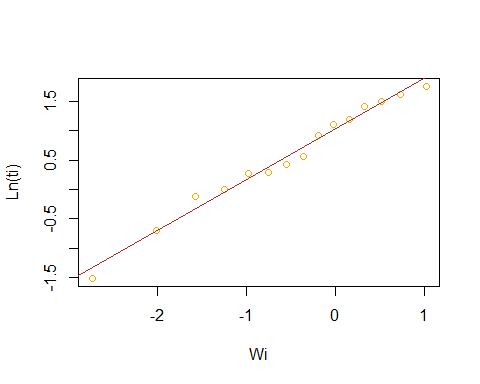
\includegraphics{M.Atighi-Project_files/figure-latex/unnamed-chunk-2-1.pdf}
According to the above figure we can see that we had three times high
loss values which are more than 100.

\subsection{Histogram Plot of Data}\label{histogram-plot-of-data}

Now we want to see the histogram plot of Data (Loss Values) to recive an
interview of loss density.

\begin{Shaded}
\begin{Highlighting}[]
\FunctionTok{ggplot}\NormalTok{(danishuni, }\FunctionTok{aes}\NormalTok{(}\AttributeTok{x =}\NormalTok{ Loss)) }\SpecialCharTok{+}
  \FunctionTok{geom\_histogram}\NormalTok{(}\AttributeTok{binwidth =} \DecValTok{3}\NormalTok{, }\AttributeTok{fill =} \DecValTok{85}\NormalTok{, }\AttributeTok{alpha =} \FloatTok{0.7}\NormalTok{ , }\AttributeTok{color =} \StringTok{"black"}\NormalTok{) }\SpecialCharTok{+}
  \FunctionTok{labs}\NormalTok{(}\AttributeTok{title =} \StringTok{"Distribution of Total Losses"}\NormalTok{, }\AttributeTok{x =} \StringTok{"Loss (mDKK)"}\NormalTok{, }\AttributeTok{y =} \StringTok{"Frequency"}\NormalTok{)}
\end{Highlighting}
\end{Shaded}

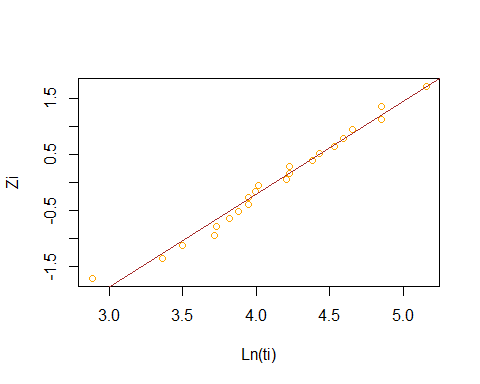
\includegraphics{M.Atighi-Project_files/figure-latex/unnamed-chunk-3-1.pdf}
According to the above Figure we can see that Loss values following very
heavy tail distribution. it means that we can see very huge loss values
in the histogram at right side of that.

\subsection{Histogram of Transformation data
(ln)}\label{histogram-of-transformation-data-ln}

for better interview we can use a transformation like ln from the loss
values, then we can again draw the histogram plot. in the following
figure we can see that.

\begin{Shaded}
\begin{Highlighting}[]
\FunctionTok{ggplot}\NormalTok{(danishuni, }\FunctionTok{aes}\NormalTok{(}\AttributeTok{x =} \FunctionTok{log}\NormalTok{(Loss))) }\SpecialCharTok{+}
  \FunctionTok{geom\_histogram}\NormalTok{(}\AttributeTok{binwidth =} \FloatTok{0.1}\NormalTok{, }\AttributeTok{fill =} \DecValTok{85}\NormalTok{, }\AttributeTok{alpha =} \FloatTok{0.7}\NormalTok{ , }\AttributeTok{color =} \StringTok{"black"}\NormalTok{) }\SpecialCharTok{+}
  \FunctionTok{labs}\NormalTok{(}\AttributeTok{title =} \StringTok{"Distribution of log of Total Losses"}\NormalTok{, }\AttributeTok{x =} \StringTok{"ln(Loss) (mDKK)"}\NormalTok{, }\AttributeTok{y =} \StringTok{"Frequency"}\NormalTok{)}
\end{Highlighting}
\end{Shaded}

\includegraphics{M.Atighi-Project_files/figure-latex/unnamed-chunk-4-1.pdf}
Like as the first histogram we can see again a heavy tail distribution
for ln(loss). it means that the loss distributions is probably pareto or
exponential.

\subsection{Mean Excess Plot of Data}\label{mean-excess-plot-of-data}

According to the histogram of the Loss values. we are going to draw Mean
Excess Plot which we can see that:(attention that i found two code for
this drawing. but i use on of them and the other one is commented in my
codes.)

\begin{Shaded}
\begin{Highlighting}[]
\CommentTok{\# Load the dataset}
\CommentTok{\# Assuming your dataset is a data frame with columns \textquotesingle{}date\textquotesingle{} and \textquotesingle{}loss\textquotesingle{}}
\CommentTok{\# Example of loading a dataset:}
\FunctionTok{library}\NormalTok{(fitdistrplus)}
\end{Highlighting}
\end{Shaded}

\begin{Shaded}
\begin{Highlighting}[]
\FunctionTok{data}\NormalTok{(}\StringTok{"danishuni"}\NormalTok{)}

\CommentTok{\# Extract the \textquotesingle{}loss\textquotesingle{} column}
\NormalTok{loss\_data }\OtherTok{\textless{}{-}}\NormalTok{ danishuni}\SpecialCharTok{$}\NormalTok{Loss}

\CommentTok{\# Sort the loss data}
\NormalTok{n }\OtherTok{\textless{}{-}} \FunctionTok{length}\NormalTok{(loss\_data)}
\NormalTok{sorted\_data }\OtherTok{\textless{}{-}} \FunctionTok{sort}\NormalTok{(loss\_data)}

\CommentTok{\# Function to calculate the mean excess for a given k}
\NormalTok{mean\_excess }\OtherTok{\textless{}{-}} \ControlFlowTok{function}\NormalTok{(data, k) \{}
\NormalTok{  threshold }\OtherTok{\textless{}{-}}\NormalTok{ data[k]}
\NormalTok{  excesses }\OtherTok{\textless{}{-}}\NormalTok{ data[(k}\SpecialCharTok{+}\DecValTok{1}\NormalTok{)}\SpecialCharTok{:}\NormalTok{n] }\SpecialCharTok{{-}}\NormalTok{ threshold}
  \FunctionTok{return}\NormalTok{(}\FunctionTok{mean}\NormalTok{(excesses, }\AttributeTok{na.rm =} \ConstantTok{TRUE}\NormalTok{))}
\NormalTok{\}}

\CommentTok{\# Compute the mean excess values for each k}
\NormalTok{mean\_excess\_values }\OtherTok{\textless{}{-}} \FunctionTok{sapply}\NormalTok{(}\DecValTok{1}\SpecialCharTok{:}\NormalTok{(n}\DecValTok{{-}1}\NormalTok{), }\ControlFlowTok{function}\NormalTok{(k) }\FunctionTok{mean\_excess}\NormalTok{(sorted\_data, k))}

\CommentTok{\# Prepare points for the plot}
\NormalTok{x\_points }\OtherTok{\textless{}{-}}\NormalTok{ sorted\_data[}\DecValTok{1}\SpecialCharTok{:}\NormalTok{(n}\DecValTok{{-}1}\NormalTok{)] }\CommentTok{\# X\_\{k,n\}}
\NormalTok{y\_points }\OtherTok{\textless{}{-}}\NormalTok{ mean\_excess\_values   }\CommentTok{\# e\_n(X\_\{k,n\})}

\CommentTok{\# Create the Mean Excess Plot}
\FunctionTok{plot}\NormalTok{(x\_points, y\_points, }\AttributeTok{type =} \StringTok{"p"}\NormalTok{, }\AttributeTok{pch =} \DecValTok{16}\NormalTok{, }\AttributeTok{col =} \StringTok{"blue"}\NormalTok{,}
     \AttributeTok{xlab =} \StringTok{"Threshold (X\_\{k,n\})"}\NormalTok{,}
     \AttributeTok{ylab =} \StringTok{"Mean Excess e\_n(X\_\{k,n\})"}\NormalTok{,}
     \AttributeTok{main =} \StringTok{"Mean Excess Plot"} 
    \CommentTok{\#, xlim = c(0 , 70)}
\NormalTok{     )}
\FunctionTok{abline}\NormalTok{(}\AttributeTok{h =} \DecValTok{0}\NormalTok{, }\AttributeTok{col =} \StringTok{"red"}\NormalTok{, }\AttributeTok{lty =} \DecValTok{2}\NormalTok{)}
\end{Highlighting}
\end{Shaded}

\includegraphics{M.Atighi-Project_files/figure-latex/unnamed-chunk-6-1.pdf}

\begin{Shaded}
\begin{Highlighting}[]
\CommentTok{\# library(fExtremes)}
\CommentTok{\# mePlot(danishuni$Loss)}
\end{Highlighting}
\end{Shaded}

The Mean Excess Plot you provided shows the behavior of the \textbf{mean
excess function} for varying thresholds. Here's an analysis of the plot:

\begin{enumerate}
\def\labelenumi{\arabic{enumi}.}
\tightlist
\item
  \textbf{Axes Explanation}:

  \begin{itemize}
  \tightlist
  \item
    The \textbf{x-axis} represents the threshold (\(X_{k,n}\)), which is
    the value above which we calculate the mean excess.
  \item
    The \textbf{y-axis} represents the \textbf{mean excess values}
    (\(e_n(X_{k,n})\)), which are the average values of data points
    exceeding each threshold.
  \end{itemize}
\item
  \textbf{Shape of the Curve}:

  \begin{itemize}
  \tightlist
  \item
    The plot starts with a rising trend at lower thresholds. This
    indicates that as we increase the threshold, the average excess
    values also increase.
  \item
    Beyond a certain threshold (approximately \(X \approx 50\)), the
    plot becomes nearly linear, which suggests that the data beyond this
    point might follow a \textbf{Generalized Pareto Distribution (GPD)}.
  \item
    At higher thresholds (e.g., \(X > 100\)), there are fewer points,
    and the variability increases due to fewer observations exceeding
    these thresholds.
  \end{itemize}
\item
  \textbf{Flatness of the Tail}:

  \begin{itemize}
  \tightlist
  \item
    If the mean excess plot exhibits a linear behavior beyond a specific
    threshold, it confirms the suitability of the GPD for modeling the
    tail.
  \item
    The almost straight-line behavior in the range \(50 < X < 100\)
    supports the GPD assumption.
  \end{itemize}
\item
  \textbf{Outliers}:

  \begin{itemize}
  \tightlist
  \item
    The last few points on the plot (e.g., \(X > 120\)) deviate
    significantly, which could be outliers or due to the sparsity of
    data in this extreme region.
  \end{itemize}
\end{enumerate}

\subsubsection{Key Observations:}\label{key-observations}

\begin{itemize}
\tightlist
\item
  \textbf{Threshold Selection}:

  \begin{itemize}
  \tightlist
  \item
    A threshold of around 50 appears reasonable because the mean excess
    function becomes nearly linear from this point onward.
  \item
    Thresholds lower than this may include non-tail behavior, which
    could bias the tail analysis.
  \end{itemize}
\item
  \textbf{Heaviness of the Tail}:

  \begin{itemize}
  \tightlist
  \item
    The increasing trend of the mean excess function indicates a
    \textbf{heavy-tailed distribution}. This is typical of datasets in
    fields like insurance and finance, where extreme values (large
    losses) are common.
  \end{itemize}
\item
  \textbf{Practical Implication}:

  \begin{itemize}
  \tightlist
  \item
    Selecting the threshold around \(X = 50\) would allow you to focus
    on the extremes while maintaining enough data points for reliable
    parameter estimation.
  \end{itemize}
\end{itemize}

\subsection{Quantile-Quantile Plot of Data with Exponential
Distribution}\label{quantile-quantile-plot-of-data-with-exponential-distribution}

According to the our goal, we need to draw the QQ plot of Loss values
with heavy tail distributions, for example here we do this work with
exponential distribution. but you should attention that we set two
lambda here, the first one is 1/mean(loss values) and the second is
1/Quantile 0.975 of loss values so we have:

\begin{Shaded}
\begin{Highlighting}[]
\CommentTok{\# Extract the \textquotesingle{}loss\textquotesingle{} column}
\FunctionTok{library}\NormalTok{(fitdistrplus)}
\FunctionTok{data}\NormalTok{(}\StringTok{"danishuni"}\NormalTok{)}
\end{Highlighting}
\end{Shaded}

\begin{Shaded}
\begin{Highlighting}[]
\NormalTok{loss\_data }\OtherTok{\textless{}{-}}\NormalTok{ danishuni}\SpecialCharTok{$}\NormalTok{Loss}

\CommentTok{\# Sort the loss data}
\NormalTok{sorted\_loss }\OtherTok{\textless{}{-}} \FunctionTok{sort}\NormalTok{(loss\_data)}

\CommentTok{\# Generate theoretical quantiles for an exponential distribution}
\NormalTok{lambda1 }\OtherTok{\textless{}{-}} \DecValTok{1}\SpecialCharTok{/}\FunctionTok{mean}\NormalTok{(loss\_data)}\CommentTok{\#quantile(loss\_data , probs = 0.975) \# Estimate rate parameter (lambda) from the data}
\NormalTok{lambda2 }\OtherTok{\textless{}{-}} \DecValTok{1}\SpecialCharTok{/}\FunctionTok{quantile}\NormalTok{(loss\_data , }\AttributeTok{probs =} \FloatTok{0.975}\NormalTok{) }\CommentTok{\# Estimate rate parameter (lambda) from the data}

\NormalTok{n }\OtherTok{\textless{}{-}} \FunctionTok{length}\NormalTok{(sorted\_loss)}
\NormalTok{exp\_quantiles1 }\OtherTok{\textless{}{-}} \FunctionTok{qexp}\NormalTok{(}\FunctionTok{ppoints}\NormalTok{(n), }\AttributeTok{rate =}\NormalTok{ lambda1)  }\CommentTok{\# Theoretical quantiles}
\NormalTok{exp\_quantiles2 }\OtherTok{\textless{}{-}} \FunctionTok{qexp}\NormalTok{(}\FunctionTok{ppoints}\NormalTok{(n), }\AttributeTok{rate =}\NormalTok{ lambda2)  }\CommentTok{\# Theoretical quantiles}

\CommentTok{\# Create the QQ{-}plot}
\FunctionTok{par}\NormalTok{(}\AttributeTok{mfrow =} \FunctionTok{c}\NormalTok{(}\DecValTok{1}\NormalTok{,}\DecValTok{2}\NormalTok{))}
\FunctionTok{qqplot}\NormalTok{(}\AttributeTok{y =}\NormalTok{ exp\_quantiles1, }\AttributeTok{x =}\NormalTok{ sorted\_loss, }
       \AttributeTok{main =} \StringTok{"QQ{-}Plot with lambda = 1/mean"}\NormalTok{,}
       \AttributeTok{xlab =} \StringTok{"Theoretical Quantiles (Exponential)"}\NormalTok{,}
       \AttributeTok{ylab =} \StringTok{"Empirical Quantiles (Loss)"}\NormalTok{,}
       \AttributeTok{pch =} \DecValTok{16}\NormalTok{, }\AttributeTok{col =} \StringTok{"blue"}\NormalTok{)}
\CommentTok{\# Add a 45{-}degree reference line}
\FunctionTok{abline}\NormalTok{(}\DecValTok{0}\NormalTok{, }\DecValTok{1}\NormalTok{, }\AttributeTok{col =} \StringTok{"red"}\NormalTok{, }\AttributeTok{lty =} \DecValTok{2}\NormalTok{)}
\CommentTok{\#add second plot }
\FunctionTok{qqplot}\NormalTok{(}\AttributeTok{y =}\NormalTok{ exp\_quantiles2, }\AttributeTok{x =}\NormalTok{ sorted\_loss, }
       \AttributeTok{main =} \StringTok{"QQ{-}Plot with lambda = 1/percentile(0.975)"}\NormalTok{,}
       \AttributeTok{xlab =} \StringTok{"Theoretical Quantiles (Exponential)"}\NormalTok{,}
       \AttributeTok{ylab =} \StringTok{"Empirical Quantiles (Loss)"}\NormalTok{,}
       \AttributeTok{pch =} \DecValTok{16}\NormalTok{, }\AttributeTok{col =} \StringTok{"blue"}\NormalTok{)}
\CommentTok{\# Add a 45{-}degree reference line}
\FunctionTok{abline}\NormalTok{(}\DecValTok{0}\NormalTok{, }\DecValTok{1}\NormalTok{, }\AttributeTok{col =} \StringTok{"red"}\NormalTok{, }\AttributeTok{lty =} \DecValTok{2}\NormalTok{)}
\end{Highlighting}
\end{Shaded}

\includegraphics{M.Atighi-Project_files/figure-latex/unnamed-chunk-8-1.pdf}
QQ-Plot with Lambda = 1/Mean The left QQ-Plot shows the empirical
quantiles of the loss data against the theoretical quantiles of an
exponential distribution with a lambda equal to the inverse of the mean
of the data. In this plot:

The data points should ideally follow the 1-1 line if the data fits the
exponential distribution well.

The regression line provides a visual indication of the overall trend.

The 95\% confidence bar helps visualize the variability around the
theoretical quantiles.

In this case, if the data points deviate significantly from the 1-1
line, especially at higher quantiles, it suggests that the loss data has
a heavier tail than what would be expected under an exponential
distribution with this lambda value.

QQ-Plot with Lambda = 1/Percentile(0.975) The right QQ-Plot uses a
lambda value set to the inverse of the 99th percentile of the data. This
can sometimes provide a better fit for the extreme values. In this plot:

Similarly, data points should follow the 1-1 line for a good fit.

The regression line and 95\% confidence bar provide additional context.

Again, if the data points, particularly at the higher end, deviate from
the 1-1 line, it indicates that the loss data has a heavy tail, which
means it has higher probabilities for extreme values compared to the
exponential distribution with the given lambda. So we can say
that:\textbackslash{} From both plots, if you observe a consistent
pattern where the empirical quantiles are above the theoretical
quantiles at higher values, it indeed suggests that your data has a
heavy tail. This means that extreme losses are more frequent in your
dataset than what would be expected from a simple exponential
distribution.

Heavy tails are common in financial and insurance datasets, and they
often require distributions that can model extreme events more
accurately, such as the Generalized Pareto Distribution (GPD) or the
Generalized Extreme Value (GEV) distribution.

\subsection{Quantile-Quantile Plot of Data with Pareto
Distribution}\label{quantile-quantile-plot-of-data-with-pareto-distribution}

According to the our goal, we need to draw the QQ plot of Loss values
with more heavy tail distributions, for example here we do this work
with pareto distribution which the sigma and alpha parameter is set as
bottem. so we have:

\begin{Shaded}
\begin{Highlighting}[]
\CommentTok{\# Load the dataset}
\FunctionTok{library}\NormalTok{(fitdistrplus)}
\FunctionTok{data}\NormalTok{(}\StringTok{"danishuni"}\NormalTok{)}
\end{Highlighting}
\end{Shaded}

\begin{Shaded}
\begin{Highlighting}[]
\NormalTok{loss\_data }\OtherTok{\textless{}{-}}\NormalTok{ danishuni}\SpecialCharTok{$}\NormalTok{Loss}

\CommentTok{\# Sort the loss data}
\NormalTok{sorted\_loss }\OtherTok{\textless{}{-}} \FunctionTok{sort}\NormalTok{(loss\_data)}
\NormalTok{n }\OtherTok{\textless{}{-}} \FunctionTok{length}\NormalTok{(sorted\_loss)}

\CommentTok{\# Estimate Pareto parameters}
\CommentTok{\# We\textquotesingle{}ll estimate the scale (sigma) and shape (alpha) using the method of moments}
\NormalTok{sigma }\OtherTok{\textless{}{-}} \FunctionTok{min}\NormalTok{(loss\_data)  }\CommentTok{\# Scale parameter (minimum value of the data)}
\NormalTok{alpha }\OtherTok{\textless{}{-}} \DecValTok{1} \SpecialCharTok{/}\NormalTok{ (}\FunctionTok{log}\NormalTok{(}\FunctionTok{mean}\NormalTok{(loss\_data }\SpecialCharTok{/}\NormalTok{ sigma)))  }\CommentTok{\# Shape parameter}

\CommentTok{\# Generate theoretical quantiles for the Pareto distribution}
\NormalTok{pp }\OtherTok{\textless{}{-}} \FunctionTok{ppoints}\NormalTok{(n)  }\CommentTok{\# Proportions for quantiles}
\NormalTok{pareto\_quantiles }\OtherTok{\textless{}{-}}\NormalTok{ sigma }\SpecialCharTok{*}\NormalTok{ (}\DecValTok{1} \SpecialCharTok{{-}}\NormalTok{ pp)}\SpecialCharTok{\^{}}\NormalTok{(}\SpecialCharTok{{-}}\DecValTok{1} \SpecialCharTok{/}\NormalTok{ alpha)  }\CommentTok{\# Theoretical quantiles}

\CommentTok{\# Create the QQ{-}plot}
\FunctionTok{par}\NormalTok{(}\AttributeTok{mfrow =} \FunctionTok{c}\NormalTok{(}\DecValTok{1}\NormalTok{,}\DecValTok{1}\NormalTok{))}
\FunctionTok{qqplot}\NormalTok{(}\AttributeTok{y =}\NormalTok{ pareto\_quantiles, }\AttributeTok{x =}\NormalTok{ sorted\_loss, }
       \AttributeTok{main =} \StringTok{"QQ{-}Plot of Loss Data vs Pareto Distribution"}\NormalTok{,}
       \AttributeTok{xlab =} \StringTok{"Theoretical Quantiles (Pareto)"}\NormalTok{,}
       \AttributeTok{ylab =} \StringTok{"Empirical Quantiles (Loss)"}\NormalTok{,}
       \AttributeTok{pch =} \DecValTok{16}\NormalTok{, }\AttributeTok{col =} \StringTok{"blue"}\NormalTok{)}
\CommentTok{\# Add a 45{-}degree reference line}
\FunctionTok{abline}\NormalTok{(}\DecValTok{0}\NormalTok{, }\DecValTok{1}\NormalTok{, }\AttributeTok{col =} \StringTok{"red"}\NormalTok{, }\AttributeTok{lty =} \DecValTok{2}\NormalTok{)}
\end{Highlighting}
\end{Shaded}

\includegraphics{M.Atighi-Project_files/figure-latex/unnamed-chunk-10-1.pdf}

From examining the QQ-Plot, there are a few key points we can discuss
about the data and its fit to the Pareto distribution:\textbackslash{}
The data points closely follow the 1-1 line at the lower quantiles. This
indicates a
\textbf{good fit to the Pareto distribution in the lower quantile range, meaning that the majority of your loss data aligns well with this distribution}.
At the higher quantiles, however, the data points begin to deviate
significantly from the 1-1 line. This suggests that the Pareto
distribution may not adequately capture the extreme values in your
dataset. The deviations at higher quantiles confirm that your dataset
has a heavy tail, where extreme losses occur more frequently than would
be expected under the Pareto distribution. This is an important
characteristic in risk management and financial modeling. Given the
heavy tail in your data, you might consider fitting your data to
distributions specifically designed to handle extreme values, such as
the Generalized Pareto Distribution (GPD) or the Generalized Extreme
Value (GEV) distribution.

\subsection{Gumbels Method of
Exceedances}\label{gumbels-method-of-exceedances}

\begin{Shaded}
\begin{Highlighting}[]
\FunctionTok{library}\NormalTok{(dplyr)}
\NormalTok{n }\OtherTok{=} \FunctionTok{nrow}\NormalTok{(danishuni)}
\NormalTok{r }\OtherTok{=} \DecValTok{25}
\NormalTok{j }\OtherTok{=} \DecValTok{0}\SpecialCharTok{:}\DecValTok{9}
\NormalTok{df }\OtherTok{=} \FunctionTok{data.frame}\NormalTok{(}\AttributeTok{probability =} \DecValTok{0}\SpecialCharTok{:}\DecValTok{9}\NormalTok{)}
\NormalTok{k\_max }\OtherTok{=} \FunctionTok{length}\NormalTok{(}\FunctionTok{which}\NormalTok{(danishuni}\SpecialCharTok{$}\NormalTok{Loss }\SpecialCharTok{\textgreater{}=} \FunctionTok{quantile}\NormalTok{(danishuni}\SpecialCharTok{$}\NormalTok{Loss , }\FloatTok{0.95}\NormalTok{)))}

\ControlFlowTok{for}\NormalTok{(k }\ControlFlowTok{in} \DecValTok{1}\SpecialCharTok{:}\NormalTok{k\_max)\{}
\NormalTok{  df1 }\OtherTok{=} \FunctionTok{data.frame}\NormalTok{(}\AttributeTok{K =} \FunctionTok{round}\NormalTok{( }\FunctionTok{choose}\NormalTok{((r }\SpecialCharTok{+}\NormalTok{ n }\SpecialCharTok{{-}}\NormalTok{ k }\SpecialCharTok{{-}}\NormalTok{ j) , (n}\SpecialCharTok{{-}}\NormalTok{k) ) }\SpecialCharTok{*} \FunctionTok{choose}\NormalTok{((j }\SpecialCharTok{+}\NormalTok{ k }\SpecialCharTok{{-}} \DecValTok{1}\NormalTok{) , (k}\DecValTok{{-}1}\NormalTok{) ) }\SpecialCharTok{/} \FunctionTok{choose}\NormalTok{((r }\SpecialCharTok{+}\NormalTok{ n ) , (n) )  , }\DecValTok{4}\NormalTok{))}
\NormalTok{  df }\OtherTok{\textless{}{-}} \FunctionTok{bind\_cols}\NormalTok{(df , df1)}
  
\NormalTok{\}}
\NormalTok{df }\OtherTok{=}\NormalTok{ df[,}\SpecialCharTok{{-}}\DecValTok{1}\NormalTok{]}
\end{Highlighting}
\end{Shaded}

\begin{Shaded}
\begin{Highlighting}[]
\FunctionTok{rownames}\NormalTok{(df) }\OtherTok{=} \FunctionTok{c}\NormalTok{(}\FunctionTok{paste0}\NormalTok{(}\StringTok{"j = "}\NormalTok{ , }\DecValTok{0}\SpecialCharTok{:}\DecValTok{9}\NormalTok{))}
\FunctionTok{colnames}\NormalTok{(df) }\OtherTok{=} \FunctionTok{c}\NormalTok{(}\FunctionTok{paste0}\NormalTok{(}\StringTok{"k = "}\NormalTok{ , }\DecValTok{1}\SpecialCharTok{:}\NormalTok{k\_max))}
\NormalTok{df[}\DecValTok{1}\SpecialCharTok{:}\DecValTok{9}\NormalTok{,}\DecValTok{1}\SpecialCharTok{:}\DecValTok{5}\NormalTok{]}
\end{Highlighting}
\end{Shaded}

\begin{verbatim}
##        k = 1  k = 2  k = 3  k = 4  k = 5
## j = 0 0.9886 0.9773 0.9662 0.9551 0.9442
## j = 1 0.0113 0.0223 0.0331 0.0437 0.0540
## j = 2 0.0001 0.0004 0.0007 0.0012 0.0018
## j = 3 0.0000 0.0000 0.0000 0.0000 0.0000
## j = 4 0.0000 0.0000 0.0000 0.0000 0.0000
## j = 5 0.0000 0.0000 0.0000 0.0000 0.0000
## j = 6 0.0000 0.0000 0.0000 0.0000 0.0000
## j = 7 0.0000 0.0000 0.0000 0.0000 0.0000
## j = 8 0.0000 0.0000 0.0000 0.0000 0.0000
\end{verbatim}

\subsection{The Return Period}\label{the-return-period}

\begin{Shaded}
\begin{Highlighting}[]
\NormalTok{k }\OtherTok{=} \DecValTok{100}
\NormalTok{u }\OtherTok{=} \FloatTok{10.58} \CommentTok{\# or you can use this: sort(danishuni$Loss , decreasing = T)[k]}
\NormalTok{p }\OtherTok{=} \FunctionTok{as.numeric}\NormalTok{(}\FunctionTok{substr}\NormalTok{(}\FunctionTok{names}\NormalTok{(}\FunctionTok{which.min}\NormalTok{(}\FunctionTok{abs}\NormalTok{(u }\SpecialCharTok{{-}} \FunctionTok{quantile}\NormalTok{(danishuni}\SpecialCharTok{$}\NormalTok{Loss , }\AttributeTok{probs =} \FunctionTok{seq}\NormalTok{(}\AttributeTok{from =} \DecValTok{0}\NormalTok{ , }\AttributeTok{to =} \DecValTok{1}\NormalTok{ , }\FloatTok{0.001}\NormalTok{))))) , }\DecValTok{1}\NormalTok{ , }\DecValTok{4}\NormalTok{))}\SpecialCharTok{/}\DecValTok{100}
\NormalTok{r\_k }\OtherTok{=} \FunctionTok{sum}\NormalTok{((}\DecValTok{1} \SpecialCharTok{{-}}\NormalTok{ p)}\SpecialCharTok{\^{}}\NormalTok{(}\DecValTok{1}\SpecialCharTok{:}\NormalTok{(k}\DecValTok{{-}1}\NormalTok{))) }\SpecialCharTok{*}\NormalTok{ p}
\NormalTok{r\_k}
\end{Highlighting}
\end{Shaded}

\begin{verbatim}
## [1] 0.046
\end{verbatim}

\subsection{Records as an Exploratory
Tool}\label{records-as-an-exploratory-tool}

\begin{Shaded}
\begin{Highlighting}[]
\CommentTok{\# Load necessary libraries}
\FunctionTok{library}\NormalTok{(ggplot2)}
\end{Highlighting}
\end{Shaded}

\begin{Shaded}
\begin{Highlighting}[]
\CommentTok{\# Ensure your date column is in Date format (replace \textquotesingle{}Date\textquotesingle{} with the actual column name if different)}

\CommentTok{\# Find new all{-}time high loss values}
\NormalTok{data }\OtherTok{\textless{}{-}}\NormalTok{ danishuni }\SpecialCharTok{\%\textgreater{}\%}
  \FunctionTok{arrange}\NormalTok{(Date) }\SpecialCharTok{\%\textgreater{}\%}
  \FunctionTok{mutate}\NormalTok{(}\AttributeTok{is\_new\_record =} \FunctionTok{cumsum}\NormalTok{(Loss }\SpecialCharTok{==} \FunctionTok{cummax}\NormalTok{(Loss)))}

\CommentTok{\# Count the number of new records per year}
\NormalTok{new\_records\_per\_year }\OtherTok{\textless{}{-}}\NormalTok{ data }\SpecialCharTok{\%\textgreater{}\%}
  \FunctionTok{filter}\NormalTok{(is\_new\_record }\SpecialCharTok{==} \DecValTok{1}\NormalTok{) }\SpecialCharTok{\%\textgreater{}\%}
  \FunctionTok{mutate}\NormalTok{(}\AttributeTok{year =} \FunctionTok{format}\NormalTok{(Date, }\StringTok{"\%Y"}\NormalTok{)) }\SpecialCharTok{\%\textgreater{}\%}
  \FunctionTok{group\_by}\NormalTok{(year) }\SpecialCharTok{\%\textgreater{}\%}
  \FunctionTok{summarise}\NormalTok{(}\AttributeTok{count =} \FunctionTok{n}\NormalTok{())}

\CommentTok{\# Plot the number of new records per year}
\FunctionTok{ggplot}\NormalTok{(data, }\FunctionTok{aes}\NormalTok{(}\AttributeTok{x =}\NormalTok{ Date, }\AttributeTok{y =}\NormalTok{ is\_new\_record)) }\SpecialCharTok{+}
  \FunctionTok{geom\_line}\NormalTok{() }\SpecialCharTok{+}
  \FunctionTok{geom\_point}\NormalTok{() }\SpecialCharTok{+}
  \FunctionTok{labs}\NormalTok{(}\AttributeTok{title =} \StringTok{"Number of New All{-}Time High Loss Records Per Year"}\NormalTok{,}
       \AttributeTok{x =} \StringTok{"Year"}\NormalTok{,}
       \AttributeTok{y =} \StringTok{"Number of New Records"}\NormalTok{) }\SpecialCharTok{+}
  \FunctionTok{theme\_minimal}\NormalTok{()}
\end{Highlighting}
\end{Shaded}

\includegraphics{M.Atighi-Project_files/figure-latex/unnamed-chunk-15-1.pdf}

\subsection{The Ratio of Maximum and
Sum}\label{the-ratio-of-maximum-and-sum}

\begin{Shaded}
\begin{Highlighting}[]
\NormalTok{loss\_data }\OtherTok{\textless{}{-}}\NormalTok{ danishuni}\SpecialCharTok{$}\NormalTok{Loss          }\CommentTok{\# Extract the loss column}
\NormalTok{n }\OtherTok{\textless{}{-}} \FunctionTok{length}\NormalTok{(loss\_data)               }\CommentTok{\# Number of observations}

\CommentTok{\# Values of p to consider}
\NormalTok{p\_values }\OtherTok{\textless{}{-}} \FunctionTok{seq}\NormalTok{(}\DecValTok{1}\NormalTok{,}\DecValTok{4}\NormalTok{ , }\DecValTok{1}\NormalTok{)}

\CommentTok{\# Preallocate storage for R\_n(p)}
\NormalTok{R\_n\_matrix }\OtherTok{\textless{}{-}} \FunctionTok{matrix}\NormalTok{(}\ConstantTok{NA}\NormalTok{, }\AttributeTok{nrow =}\NormalTok{ n, }\AttributeTok{ncol =} \FunctionTok{length}\NormalTok{(p\_values))}
\FunctionTok{colnames}\NormalTok{(R\_n\_matrix) }\OtherTok{\textless{}{-}} \FunctionTok{paste0}\NormalTok{(}\StringTok{"p="}\NormalTok{, p\_values)}

\CommentTok{\# Calculate R\_n(p) for each value of p}
\ControlFlowTok{for}\NormalTok{ (j }\ControlFlowTok{in} \FunctionTok{seq\_along}\NormalTok{(p\_values)) \{}
\NormalTok{  p }\OtherTok{\textless{}{-}}\NormalTok{ p\_values[j]}
\NormalTok{  abs\_loss\_p }\OtherTok{\textless{}{-}} \FunctionTok{abs}\NormalTok{(loss\_data)}\SpecialCharTok{\^{}}\NormalTok{p}
  
  \ControlFlowTok{for}\NormalTok{ (i }\ControlFlowTok{in} \DecValTok{1}\SpecialCharTok{:}\NormalTok{n) \{}
\NormalTok{    S\_n }\OtherTok{\textless{}{-}} \FunctionTok{sum}\NormalTok{(abs\_loss\_p[}\DecValTok{1}\SpecialCharTok{:}\NormalTok{i])       }\CommentTok{\# Sum up to the i{-}th element}
\NormalTok{    M\_n }\OtherTok{\textless{}{-}} \FunctionTok{max}\NormalTok{(abs\_loss\_p[}\DecValTok{1}\SpecialCharTok{:}\NormalTok{i])       }\CommentTok{\# Max up to the i{-}th element}
\NormalTok{    R\_n\_matrix[i, j] }\OtherTok{\textless{}{-}}\NormalTok{ M\_n }\SpecialCharTok{/}\NormalTok{ S\_n     }\CommentTok{\# Ratio}
\NormalTok{  \}}
\NormalTok{\}}

\CommentTok{\# Plot R\_n(p) against n for each p}
\FunctionTok{par}\NormalTok{(}\AttributeTok{mfrow =} \FunctionTok{c}\NormalTok{((}\FunctionTok{round}\NormalTok{(}\FunctionTok{length}\NormalTok{(p\_values)}\SpecialCharTok{/}\DecValTok{2}\NormalTok{ , }\DecValTok{0}\NormalTok{)), }\DecValTok{2}\NormalTok{))  }\CommentTok{\# One plot for each p}
\ControlFlowTok{for}\NormalTok{ (j }\ControlFlowTok{in} \FunctionTok{seq\_along}\NormalTok{(p\_values)) \{}
  \FunctionTok{plot}\NormalTok{(}\DecValTok{1}\SpecialCharTok{:}\NormalTok{n, R\_n\_matrix[, j], }\AttributeTok{type =} \StringTok{"l"}\NormalTok{, }
       \AttributeTok{main =} \FunctionTok{paste}\NormalTok{(}\StringTok{"R\_n(p) for p ="}\NormalTok{, p\_values[j]),}
       \AttributeTok{xlab =} \StringTok{"n"}\NormalTok{, }\AttributeTok{ylab =} \StringTok{"R\_n(p)"}\NormalTok{, }\AttributeTok{col =} \StringTok{"blue"}\NormalTok{, }\AttributeTok{lwd =} \DecValTok{2}\NormalTok{)}
  \FunctionTok{abline}\NormalTok{(}\AttributeTok{h =} \DecValTok{0}\NormalTok{, }\AttributeTok{col =} \StringTok{"red"}\NormalTok{, }\AttributeTok{lty =} \DecValTok{2}\NormalTok{) }\CommentTok{\# Add reference line at 0}
\NormalTok{\}}
\end{Highlighting}
\end{Shaded}

\includegraphics{M.Atighi-Project_files/figure-latex/unnamed-chunk-16-1.pdf}

\section{Parameter Estimation for the Generalised Extreme Value
Distribution
(GEV)}\label{parameter-estimation-for-the-generalised-extreme-value-distribution-gev}

\subsection{introduction}\label{introduction-2}

\begin{Shaded}
\begin{Highlighting}[]
\FunctionTok{library}\NormalTok{(fitdistrplus)}
\FunctionTok{library}\NormalTok{(ismev)       }\CommentTok{\# For GEV functions}
\FunctionTok{library}\NormalTok{(extRemes)    }\CommentTok{\# Additional extreme value analysis tools}
\FunctionTok{library}\NormalTok{(EnvStats)}
\end{Highlighting}
\end{Shaded}

\subsection{Maximum Likelihood
Estimation}\label{maximum-likelihood-estimation}

\subsubsection{for all data}\label{for-all-data}

\begin{Shaded}
\begin{Highlighting}[]
\FunctionTok{library}\NormalTok{(extRemes)    }\CommentTok{\# Additional extreme value analysis tools}
\end{Highlighting}
\end{Shaded}

\begin{Shaded}
\begin{Highlighting}[]
\CommentTok{\#GEV ON ALL DATA WITH MLE method}
\NormalTok{loss\_data }\OtherTok{\textless{}{-}}\NormalTok{ danishuni}\SpecialCharTok{$}\NormalTok{Loss}
\NormalTok{gev\_fit\_all\_data\_mle }\OtherTok{\textless{}{-}} \FunctionTok{fevd}\NormalTok{(loss\_data, }\AttributeTok{method =} \StringTok{"MLE"}\NormalTok{, }\AttributeTok{type =} \StringTok{"GEV"}\NormalTok{)}
\FunctionTok{summary}\NormalTok{(gev\_fit\_all\_data\_mle)}
\end{Highlighting}
\end{Shaded}

\begin{verbatim}
## 
## fevd(x = loss_data, type = "GEV", method = "MLE")
## 
## [1] "Estimation Method used: MLE"
## 
## 
##  Negative Log-Likelihood Value:  3392.418 
## 
## 
##  Estimated parameters:
##  location     scale     shape 
## 1.4833406 0.5928882 0.9165839 
## 
##  Standard Error Estimates:
##   location      scale      shape 
## 0.01507648 0.01865780 0.03034083 
## 
##  Estimated parameter covariance matrix.
##               location        scale         shape
## location  0.0002273004 2.389179e-04 -1.135461e-04
## scale     0.0002389179 3.481137e-04  9.290683e-05
## shape    -0.0001135461 9.290683e-05  9.205658e-04
## 
##  AIC = 6790.835 
## 
##  BIC = 6807.878
\end{verbatim}

\begin{Shaded}
\begin{Highlighting}[]
\FunctionTok{plot}\NormalTok{(gev\_fit\_all\_data\_mle)}
\end{Highlighting}
\end{Shaded}

\includegraphics{M.Atighi-Project_files/figure-latex/unnamed-chunk-19-1.pdf}

\begin{Shaded}
\begin{Highlighting}[]
\NormalTok{return\_level }\OtherTok{\textless{}{-}} \FunctionTok{return.level}\NormalTok{(gev\_fit\_all\_data\_mle, }\AttributeTok{return.period =} \DecValTok{100}\NormalTok{)}
\FunctionTok{print}\NormalTok{(return\_level)}
\end{Highlighting}
\end{Shaded}

\begin{verbatim}
## fevd(x = loss_data, type = "GEV", method = "MLE")
## get(paste("return.level.fevd.", newcl, sep = ""))(x = x, return.period = return.period)
## 
##  GEV model fitted to  loss_data  
## Data are assumed to be  stationary 
## [1] "Return Levels for period units in years"
## 100-year level 
##       44.68651
\end{verbatim}

\subsubsection{for Monthly maxima
data(BlockMaximum)}\label{for-monthly-maxima-datablockmaximum}

\begin{Shaded}
\begin{Highlighting}[]
\CommentTok{\#GEV ON BLOCK MAX DATA with MLE method}
\FunctionTok{library}\NormalTok{(dplyr)}
\end{Highlighting}
\end{Shaded}

\begin{Shaded}
\begin{Highlighting}[]
\NormalTok{danish\_block\_max }\OtherTok{\textless{}{-}}\NormalTok{ danishuni }\SpecialCharTok{\%\textgreater{}\%}
  \FunctionTok{group\_by}\NormalTok{(}\AttributeTok{year =}\NormalTok{ lubridate}\SpecialCharTok{::}\FunctionTok{year}\NormalTok{(Date)) }\SpecialCharTok{\%\textgreater{}\%}
  \FunctionTok{summarise}\NormalTok{(}\AttributeTok{MaxLoss =} \FunctionTok{max}\NormalTok{(Loss))}
\NormalTok{gev\_fit\_blockMax\_data\_mle }\OtherTok{\textless{}{-}} \FunctionTok{fevd}\NormalTok{(danish\_block\_max}\SpecialCharTok{$}\NormalTok{MaxLoss, }\AttributeTok{method =} \StringTok{"MLE"}\NormalTok{  , }\AttributeTok{type =} \StringTok{"GEV"}\NormalTok{)}
\FunctionTok{summary}\NormalTok{(gev\_fit\_blockMax\_data\_mle)}
\end{Highlighting}
\end{Shaded}

\begin{verbatim}
## 
## fevd(x = danish_block_max$MaxLoss, type = "GEV", method = "MLE")
## 
## [1] "Estimation Method used: MLE"
## 
## 
##  Negative Log-Likelihood Value:  58.23331 
## 
## 
##  Estimated parameters:
##   location      scale      shape 
## 37.8259460 28.9673297  0.6380642 
## 
##  Standard Error Estimates:
##   location      scale      shape 
## 10.7251910 11.0547413  0.4140545 
## 
##  Estimated parameter covariance matrix.
##            location       scale      shape
## location 115.029722  95.6378074 -1.6604664
## scale     95.637807 122.2073057 -0.1589988
## shape     -1.660466  -0.1589988  0.1714411
## 
##  AIC = 122.4666 
## 
##  BIC = 123.6603
\end{verbatim}

\begin{Shaded}
\begin{Highlighting}[]
\FunctionTok{plot}\NormalTok{(gev\_fit\_blockMax\_data\_mle)}
\end{Highlighting}
\end{Shaded}

\includegraphics{M.Atighi-Project_files/figure-latex/unnamed-chunk-21-1.pdf}

\begin{Shaded}
\begin{Highlighting}[]
\NormalTok{return\_level }\OtherTok{\textless{}{-}} \FunctionTok{return.level}\NormalTok{(gev\_fit\_blockMax\_data\_mle, }\AttributeTok{return.period =} \DecValTok{100}\NormalTok{)}
\FunctionTok{print}\NormalTok{(return\_level)}
\end{Highlighting}
\end{Shaded}

\begin{verbatim}
## fevd(x = danish_block_max$MaxLoss, type = "GEV", method = "MLE")
## get(paste("return.level.fevd.", newcl, sep = ""))(x = x, return.period = return.period)
## 
##  GEV model fitted to  danish_block_max$MaxLoss  
## Data are assumed to be  stationary 
## [1] "Return Levels for period units in years"
## 100-year level 
##        847.063
\end{verbatim}

\subsection{Method of Probability Weighted
Moments}\label{method-of-probability-weighted-moments}

\subsubsection{introduction}\label{introduction-3}

\subsubsection{for all data}\label{for-all-data-1}

\begin{Shaded}
\begin{Highlighting}[]
\NormalTok{loss\_data }\OtherTok{\textless{}{-}}\NormalTok{ danishuni}\SpecialCharTok{$}\NormalTok{Loss}
\NormalTok{gev\_fit\_all\_data\_pwm }\OtherTok{\textless{}{-}}\FunctionTok{egevd}\NormalTok{(loss\_data, }\AttributeTok{method =} \StringTok{"pwme"}\NormalTok{)}

\NormalTok{gev\_fit\_all\_data\_pwm}
\end{Highlighting}
\end{Shaded}

\begin{verbatim}
## 
## Results of Distribution Parameter Estimation
## --------------------------------------------
## 
## Assumed Distribution:            Generalized Extreme Value
## 
## Estimated Parameter(s):          location =  1.5551821
##                                  scale    =  0.7156472
##                                  shape    = -0.6709899
## 
## Estimation Method:               Unbiased pwme
## 
## Data:                            loss_data
## 
## Sample Size:                     2167
\end{verbatim}

\subsubsection{for Monthly maxima
data(BlockMaximum)}\label{for-monthly-maxima-datablockmaximum-1}

\begin{Shaded}
\begin{Highlighting}[]
\CommentTok{\#GEV ON BLOCK MAX DATA WITH PWM method}
\NormalTok{gev\_fit\_BlockMax\_pwm }\OtherTok{\textless{}{-}}\FunctionTok{egevd}\NormalTok{(danish\_block\_max}\SpecialCharTok{$}\NormalTok{MaxLoss, }\AttributeTok{method =} \StringTok{"pwme"}\NormalTok{)}
\NormalTok{gev\_fit\_BlockMax\_pwm}
\end{Highlighting}
\end{Shaded}

\begin{verbatim}
## 
## Results of Distribution Parameter Estimation
## --------------------------------------------
## 
## Assumed Distribution:            Generalized Extreme Value
## 
## Estimated Parameter(s):          location = 39.0416710
##                                  scale    = 34.8869268
##                                  shape    = -0.3818574
## 
## Estimation Method:               Unbiased pwme
## 
## Data:                            danish_block_max$MaxLoss
## 
## Sample Size:                     11
\end{verbatim}

\section{Estimating Under Maximum Domain of
Attraction}\label{estimating-under-maximum-domain-of-attraction}

\subsection{Pickands's Estimator}\label{pickandss-estimator}

\begin{Shaded}
\begin{Highlighting}[]
\FunctionTok{library}\NormalTok{(fExtremes)}
\FunctionTok{library}\NormalTok{(RobExtremes)}
\FunctionTok{library}\NormalTok{(evmix)}
\end{Highlighting}
\end{Shaded}

\begin{Shaded}
\begin{Highlighting}[]
\FunctionTok{pickandsplot}\NormalTok{(danishuni}\SpecialCharTok{$}\NormalTok{Loss)}
\end{Highlighting}
\end{Shaded}

\includegraphics{M.Atighi-Project_files/figure-latex/unnamed-chunk-25-1.pdf}
\#\# Hill's Estimator

\begin{Shaded}
\begin{Highlighting}[]
\FunctionTok{hillplot}\NormalTok{(danishuni}\SpecialCharTok{$}\NormalTok{Loss)}
\end{Highlighting}
\end{Shaded}

\includegraphics{M.Atighi-Project_files/figure-latex/unnamed-chunk-26-1.pdf}
\# Fitting Excesses Over a Threshold

\subsection{Fitting the GPD}\label{fitting-the-gpd}

\subsubsection{Introduction}\label{introduction-4}

\subsubsection{Maximum Likelihood
Estimation}\label{maximum-likelihood-estimation-1}

\begin{Shaded}
\begin{Highlighting}[]
\FunctionTok{library}\NormalTok{(extRemes)    }\CommentTok{\# Additional extreme value analysis tools}
\end{Highlighting}
\end{Shaded}

\begin{Shaded}
\begin{Highlighting}[]
\NormalTok{threshold1 }\OtherTok{=} \FunctionTok{quantile}\NormalTok{(danishuni}\SpecialCharTok{$}\NormalTok{Loss , }\AttributeTok{probs =} \FloatTok{0.95}\NormalTok{)}
\NormalTok{gpd\_fit\_all\_data }\OtherTok{\textless{}{-}} \FunctionTok{fevd}\NormalTok{(loss\_data, }\AttributeTok{threshold =}\NormalTok{ threshold1, }\AttributeTok{type =} \StringTok{"GP"}\NormalTok{ , }\AttributeTok{method =} \StringTok{"MLE"}\NormalTok{)}
\FunctionTok{summary}\NormalTok{(gpd\_fit\_all\_data)}
\end{Highlighting}
\end{Shaded}

\begin{verbatim}
## 
## fevd(x = loss_data, threshold = threshold1, type = "GP", method = "MLE")
## 
## [1] "Estimation Method used: MLE"
## 
## 
##  Negative Log-Likelihood Value:  375.3185 
## 
## 
##  Estimated parameters:
##    scale    shape 
## 7.037527 0.492032 
## 
##  Standard Error Estimates:
##     scale     shape 
## 1.1177516 0.1351766 
## 
##  Estimated parameter covariance matrix.
##             scale       shape
## scale  1.24936856 -0.08119689
## shape -0.08119689  0.01827271
## 
##  AIC = 754.637 
## 
##  BIC = 760.0197
\end{verbatim}

\begin{Shaded}
\begin{Highlighting}[]
\FunctionTok{plot}\NormalTok{(gpd\_fit\_all\_data)}
\end{Highlighting}
\end{Shaded}

\includegraphics{M.Atighi-Project_files/figure-latex/unnamed-chunk-28-1.pdf}

\begin{Shaded}
\begin{Highlighting}[]
\NormalTok{return\_level }\OtherTok{\textless{}{-}} \FunctionTok{return.level}\NormalTok{(gpd\_fit\_all\_data, }\AttributeTok{return.period =} \DecValTok{100}\NormalTok{)}
\FunctionTok{print}\NormalTok{(return\_level)}
\end{Highlighting}
\end{Shaded}

\begin{verbatim}
## fevd(x = loss_data, threshold = threshold1, type = "GP", method = "MLE")
## get(paste("return.level.fevd.", newcl, sep = ""))(x = x, return.period = return.period)
## 
##  GP model fitted to  loss_data  
## Data are assumed to be  stationary 
## [1] "Return Levels for period units in years"
## 100-year level 
##       573.0964
\end{verbatim}

\begin{Shaded}
\begin{Highlighting}[]
\NormalTok{simulated\_data5 }\OtherTok{\textless{}{-}} \FunctionTok{rgev}\NormalTok{(}\DecValTok{1000}\NormalTok{, }
                        \AttributeTok{scale =}\NormalTok{ gpd\_fit\_all\_data}\SpecialCharTok{$}\NormalTok{results}\SpecialCharTok{$}\NormalTok{par[}\StringTok{"scale"}\NormalTok{], }
                        \AttributeTok{shape =}\NormalTok{ gpd\_fit\_all\_data}\SpecialCharTok{$}\NormalTok{results}\SpecialCharTok{$}\NormalTok{par[}\StringTok{"shape"}\NormalTok{])}
\FunctionTok{head}\NormalTok{(simulated\_data5)}
\end{Highlighting}
\end{Shaded}

\begin{verbatim}
## [1] -2.621188  3.594865  5.443564 -6.427475 15.745169 23.233568
\end{verbatim}

\section{Conclusion}\label{conclusion}

The Danish reinsurance dataset provides valuable insights into fire
losses and their components, making it an excellent resource for
studying loss severity distributions and extreme value theory.

\end{document}
